\documentclass[11pt,a4paper]{article}

% Packages
\usepackage[utf8]{inputenc}
\usepackage[spanish, es-tabla]{babel}
\usepackage{caption}
\usepackage{listings}
\usepackage{adjustbox}
\usepackage{enumitem}
\usepackage{boldline}
\usepackage{amssymb, amsmath,amsthm}
\usepackage[margin=1in]{geometry}
\usepackage{xcolor}
\usepackage{soul}
\usepackage{upgreek}
\usepackage{float}

% Meta
\title{Entrega 1}
\author{José Antonio Álvarez}
\date{}

% Custom
\providecommand{\abs}[1]{\lvert#1\rvert}
\setlength\parindent{0pt}
% Redefinir letra griega épsilon.
\let\epsilon\upvarepsilon
% Fracciones grandes
\newcommand\ddfrac[2]{\frac{\displaystyle #1}{\displaystyle #2}}
% Primera derivada parcial: \pder[f]{x}
\newcommand{\pder}[2][]{\frac{\partial#1}{\partial#2}}

\begin{document}

\maketitle

\textbf{Ejercicio 17.} Diseña un autómata finito determinista que reconozca el siguiente lenguaje: $$L = \{ u \in \{ 0,1\}^* \ | \ \text{el número de $1$ no es múltiplo de $3$ y el número de $0$ es par} \}$$ 

\begin{figure}[H]
	\centering
	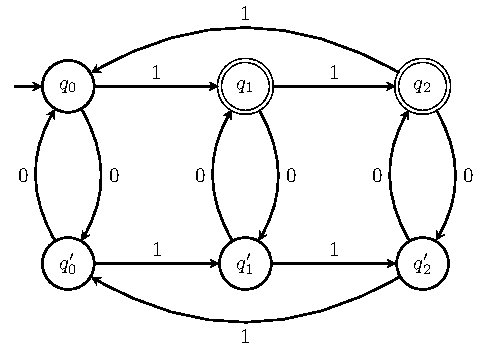
\includegraphics[width=0.8\textwidth]{afd_17}
	\caption{Autómata finito determinista que reconoce $L$.}
\end{figure}

\newpage

\textbf{Ejercicio 22.} Dar una expresión regular para el lenguaje aceptado por el siguiente autómata: \\

\begin{figure}[H]
	\centering
	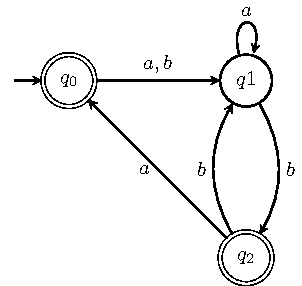
\includegraphics[width=0.8\textwidth]{afd_22_1}
	\caption{Autómata finito determinista del enunciado.}
\end{figure}

Reducimos el autómata a dos estados para estudiar $r_2$ (camino entre el estado inicial y el estado $q_2$): \\

\begin{figure}[H]
	\centering
	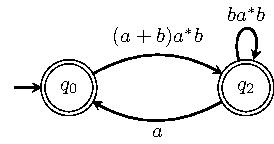
\includegraphics[width=0.8\textwidth]{afd_22_2}
	\caption{Autómata reducido a 2 estados para calcular $r_2$}
\end{figure}

La expresión resultante es la siguiente: $$r_2 = ((a+b)a^*b(ba^*b)^*a)^*(a+b)a^*b(ba^*b)^* $$ A continuación reducimos el autómata a un sólo estado y estudiamos $r_0$:

\begin{figure}[H]
	\centering
	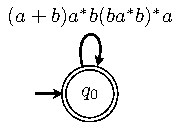
\includegraphics[width=0.8\textwidth]{afd_22_3}
	\caption{Autómata reducido a 1 estado para calcular $r_0$}
\end{figure}

$$r_0 = ((a+b)a^*b(ba^*b)^*a)^* $$

La expresión regular asociada al autómata es la suma de ambas:

$$r_0 + r_2 = ((a+b)a^*b(ba^*b)^*a)^*(a+b)a^*b(ba^*b)^* + ((a+b)a^*b(ba^*b)^*a)^* $$

\textbf{Ejercicio 23.} Sea $B_n = \{a^k \ | \ k \text{ es múltiplo de } n \}$. Demostrar que $B_n$ es regular para todo $n$.\\

Como ser lenguaje regular y obtener una expresión regular del lenguaje es equivalente, basta con hacer esto último. La expresión será $(a..(n)..a)^*$. Es decir, $n$ letras $a$'s entre paréntesis. \\



\textbf{Ejercicio 24.} Decimos que $u$ es un prefijo de $v$ si existe $w$ tal que $uw = v$. Decimos que $u$ es un prefijo propio de $v$ si además $u \neq \epsilon$ y $u \neq v$. Demostrar que si $L$ es regular, también lo son los lenguajes: 
\begin{itemize}
	\item $NOPREFIJO(L) = \{u \in L \ | \ \text{ningún prefijo propio de } u \text{ pertenece a } L\} = NP(L)$
	\item $NOEXTENSION(L) = \{u \in L \ | \ u \text{ no es un prefijo propio de ninguna palabra de } L\} = NE(L)$
\end{itemize}

Como L es un lenguaje regular, existe una gramática $G(L) = \{ (V, T, P, S) \}$ cumpliendo que todas las reglas de producción son de la forma $A \rightarrow uB$ ó $A \rightarrow u$, con $u \in T^*$ y $A,B \in V$. \\

Para mostrar que los lenguajes son regulares encontraremos unas grámaticas cumpliendo lo anterior. Para ello únicamente quitaremos reglas de producción, por lo que la gramática resultante seguirá generando un lenguaje de tipo 3. \\

Para $NP(L)$, si dado un estado $A \in V$ existen dos reglas de producción de la forma $A \rightarrow \epsilon$ y $A \rightarrow x$, con $A \rightarrow x$, eliminamos todas las reglas de la forma $x \in T^*\cup V$. \\

De forma análoga, para $NE(L)$, si dado un estado $A \in V$ existen dos reglas de producción de la forma $A \rightarrow \epsilon$ y $A \rightarrow x$, con $x \in T^*\cup V$, eliminamos todas las reglas de la forma $A \rightarrow \epsilon$. \\

Estas grámaticas nos generan los lenguajes y esto prueba que son regulares. \\

\textbf{Ejercicio 25.} Si $L \subset A^*$ , define la relación $\equiv$ en $A^*$ como sigue: si $u,v \in A^*$ , entonces $u \equiv v$ si y solo si
para toda $z \in A^*$ , tenemos que $(xz \in L \leftrightarrow yz \in L)$.
\begin{enumerate}
	\item Demostrar que $\equiv$ es una relación de equivalencia.
	
\begin{itemize}
	\item Reflexividad: $x \equiv y \leftrightarrow \forall z \in A^* \ [ \ xz \in L \leftrightarrow yz \in L \ ]$, obvio.
	\item Simetría: $x \equiv y \leftrightarrow \forall z \in A^* \ [ \ xz \in L \leftrightarrow yz \in L \ ] \leftrightarrow \forall z \in A^* \ [ \ yz \in L \leftrightarrow xz \in L \ ] \leftrightarrow y \equiv x $.
	\item Transitividad: $u,v,w\in A^*, u \equiv v, v \equiv w \rightarrow \forall z \in A^* \ [ \ uz \in L \leftrightarrow vz \in L \ ] \text{ y } [ \ vz \in L \leftrightarrow wz \in L \ ] \rightarrow\forall z \in A^* \ [ \ uz \in L \leftrightarrow wz \in L \ ] \rightarrow u \equiv w$.
\end{itemize}

	\item Calcular las clases de equivalencia de $L = \{a^ib^i | i \geq 0\}$

Hay infinitas clases de equivalencia:

\begin{itemize}
	\item Denotamos con $[noL]$ a la clase de equivalencia de todas las palabras que ni son del lenguaje ni lo serán añadiendoles elemenos. Es decir, aquellas que contienen la subcadena $ba$ o que son de la forma $a^ib^j$ con $j > i$.
	\item Cada palabra que no es de la forma anteriormente descrita tiene su propia clase de equivalencia. Esto incluye a la cadena vacía, las palabras de la forma $a^i$ y las de la forma $a^ib^j$ con $j \leq i$. Es sencillo darse cuenta de que estas son efectivamente clases de equivalencia.
\end{itemize}

	\item Calcular las clases de equivalencia de $L = \{a^ib^j | i,j \geq 0\}$
	
Hay tres clases de equivalencia:

\begin{itemize}
	\item Analogamente al apartado anterior, denotamos con $[noL]$ a la clase de equivalencia de todas las palabras que ni son del lenguaje ni lo serán añadiendoles elemenos. En este caso las únicas palabras de esta clase son las que contienen la subcadena $ba$.
	\item Sea [a] la clase de equivalencia de todas las palabras de la forma $a^i$.
	\item Por último, sea [ab] la clase de equivalencia de las palabras de la forma $a^ib^j$ con $j > 0$. Esta clase se diferencia de la clase anterior utilizando $z = ab$ en la definición de $\equiv$. 
\end{itemize}
	
	\item Demostrar que $L$ es aceptado por un autómata finito determinístico si y solo si el número de clases de equivalencia es finito.

Veamos primero la implicación hacia la derecha. 

Como $L$ es aceptado por un AFD, tomamos el autómata minimal. A continuación definimos: $$ L_{q_i} = \{ u \in A^* \ | \ \delta^*(q_0, u) = q_i \}$$

Como el número de estados es finitio, el número de $L_{q_i}$ también lo es. Veámos ahora que $\forall u \in A^* \ \exists q_i \text{ t.q. } [u] = L_{q_i} $. Esto es, el número de clases de equivalencia es el mismo que el número de estados (lo que responde al apartado \textbf{5}). Si demostramos eso, habremos demostrado que el número de clases de equivalencia es finito.

\begin{itemize}
	\item \underline{$L_{q_i} \subset [u]$} \\
	
Si $x \in L_{q_i} \rightarrow \forall z \in A^* \text{ se cumple que : } \delta^*(q_0, xz) = \delta^*(\delta^*(q_0,x), z) = \delta^*(q_i, z) = \delta^*(\delta^*(q_0,u), z) = \delta^*(q_0, uz) \rightarrow [xz \in L \leftrightarrow uz \in L] \rightarrow x \equiv u \rightarrow x \in [u]$. \\

	\item \underline{$[u] \subset L_{q_i}$} \\
	
Pequeño recordatorio: $F$ es el conjunto de estados finales del autómata.
	
Supongamos que no: $\exists v \in [u] \text{ t.q. } \delta*(q_0,v) = q_x \neq q_i$. Como $u \equiv v \rightarrow \forall z \in A^* [ \ uz \in L \leftrightarrow vz \in L \ ] \leftrightarrow [ \ \delta^*(q_0, uz) \in F \leftrightarrow \delta^*(q_0, vz) \in F \ ] \leftrightarrow [ \ \delta^*(\delta^*(q_0,u), z) \in F \leftrightarrow \delta^*(\delta^*(q_0,v), z) \in F \ ] \leftrightarrow [ \ \delta^*(q_x, z) \in F \leftrightarrow \delta^*(q_i, z) \in F \ ] \leftrightarrow q_i$ y $q_x$ son estados equivalentes. Sin embargo, estamos en un AF minimal, no hay estados equivalentes. Hemos llegado a una contradicción.
	
\end{itemize}
	
Veamos en segundo lugar la implicación hacia la izquierda. Para ello, construyamos un AFD a partir de las clases de equivalencia. Asociando a cada clase un estado obtenemos un AF ya que el número de clases de equivalencia es finito. 

Sea $q_u$ el estado asociado a la clase de equivalencia de u, $[u]$. Definimos la función de transición como $\delta(q_u, a) = q_{ua}$. Es decir, pasamos del estado asociado a $[u]$ al estado asociado a $[ua]$. Definimos el estado inicial como el estado al que pertenece la cadena vacía y los estados finales serán aquellos estados en los que las palabras de la clase de equivalencia asociada al estado sean aceptadas por el lenguaje.

Esto nos define un AFD que acepta el lenguaje.
	
	\item ¿Qué relación existe entre el número de clases de equivalencia y el autómata finito minimal que acepta $L$?

El número de clases de equivalencia es el número de estados del AF minimal asociado, como probamos en el apartado anterior.

\end{enumerate}

\end{document}